\documentclass[10pt,journal,compsoc]{IEEEtran}

\ifCLASSOPTIONcompsoc
  \usepackage[nocompress]{cite}
\else
  \usepackage{cite}
\fi

\usepackage[T1]{fontenc}
\usepackage[utf8]{inputenc}
\usepackage{amsmath,amssymb,amsfonts,amsthm}
\usepackage{mathtools}
\usepackage{graphicx}
\usepackage{booktabs}
\usepackage{multirow}
\usepackage{array}
\usepackage{xcolor}
\usepackage{microtype}
\usepackage{url}
\def\UrlBreaks{\do\/\do-\do\_\do.}
\usepackage[hidelinks]{hyperref}
\pdfstringdefDisableCommands{%
  \def\SM{SonarMoE}%
  \def\OD{OblivDispatch}%
}

\graphicspath{{figures/}}

\newtheorem{theorem}{Theorem}
\newtheorem{lemma}{Lemma}
\newtheorem{proposition}{Proposition}
\newtheorem{corollary}{Corollary}
\theoremstyle{definition}
\newtheorem{definition}{Definition}
\theoremstyle{remark}
\newtheorem{remark}{Remark}

\newcommand{\SM}{\textsc{SonarMoE}}
\newcommand{\OD}{\textsc{OblivDispatch}}
\newcommand{\MLB}{\textsc{MoELeak-Bench}}

\begin{document}

\title{SonarMoE: Remote Prompt and Tool-Schema Reconstruction via Cross-Node Expert Contention in Disaggregated MoE Serving and Differentially Private Mitigation}

\author{Mohammed~Kamran~Syed,
        Anudeep~Rentala,
        Somesh~Rahul,\\
        Raghuram~Malpe~Pai,
        and~Krishna~Suman~Dara%
\IEEEcompsocitemizethanks{%
\IEEEcompsocthanksitem M.~K.~Syed (Corresponding Author) is an IEEE Independent Researcher, Mountain House, CA, USA (e-mail: mohammedkamran.syed@ieee.org; ORCID: 0009-0009-9058-5375).
\IEEEcompsocthanksitem A.~Rentala and S.~Rahul are IEEE Independent Researchers, Fremont, CA, USA (e-mail: anudeep.rentala@ieee.org; someshrahul@ieee.org).
\IEEEcompsocthanksitem R.~M.~Pai and K.~S.~Dara are IEEE Independent Researchers, Sunnyvale, CA, USA (e-mail: raghuram.pai@ieee.org; krishna-suman.dara@ieee.org).
\IEEEcompsocthanksitem Manuscript draft, November 2026.}}

\markboth{IEEE TRANSACTIONS ON DEPENDABLE AND SECURE COMPUTING}%
{SYED ET AL.: SONARMOE: REMOTE PROMPT AND TOOL-SCHEMA RECONSTRUCTION IN DISAGGREGATED MOE SERVING}

\IEEEtitleabstractindextext{%
\begin{abstract}
Production Mixture-of-Experts serving clusters increasingly disaggregate stateful Attention frontends from shared Expert-Parallel feed-forward pools over datacenter RDMA fabrics. Cloud operators treat Attention-FFN Disaggregation as isolated against cross-tenant inference leaks because tenants run on separate Attention containers with zero shared Key-Value cache memory and zero host co-residency. We show that an external adversary holding only a standard streaming HTTP API key can still reconstruct co-scheduled victim prompt domains and Model Context Protocol tool schemas across disaggregated nodes. Our attack, SonarMoE, synthesizes rank-concentrated canary tokens offline from public router weights without victim data and sizes canary micro-batches right below discrete GPU matrix-multiply tile cliffs. Even a few co-scheduled victim tokens routed to a primed expert push execution into an additional hardware tile, producing microsecond Inter-Token Latency echoes observable over remote HTTP streams. Across OLMoE-1B-7B and Granite-3.1-MoE on Apple M5 Pro GPUs under strict constant-length controls, SonarMoE reaches 85.0 percent five-domain accuracy and 89.4 percent Top-1 accuracy across twenty MCP tool schemas, nearly doubling naive canary accuracy under network jitter. Our defense, OblivDispatch, hides shadow-expert overflow and differentially private count blinding inside cross-rank barrier slack, reducing attacker accuracy to random guessing at under 5.5 percent latency overhead.
\end{abstract}

\begin{IEEEkeywords}
Mixture-of-Experts, disaggregated LLM serving, remote timing side channels, Model Context Protocol, differential privacy, GPU tile quantization.
\end{IEEEkeywords}}

\maketitle
\IEEEdisplaynontitleabstractindextext
\IEEEpeerreviewmaketitle

% ============================================================================
\section{Introduction}\label{sec:intro}
% ============================================================================

Sparse Mixture-of-Experts (MoE) transformers decouple parameter count from per-token arithmetic by activating a small top-$k$ subset of specialized feed-forward networks (FFNs) for each token~\cite{shazeer2017outrageously,fedus2022switch}. Frontier open-weight models including \texttt{DeepSeek-V2/V3/R1}~\cite{deepseek2024v2,deepseek2025v3,deepseek2025r1}, \texttt{Qwen2-MoE}~\cite{yang2024qwen2moe}, \texttt{Mixtral}~\cite{jiang2024mixtral}, and \texttt{OLMoE}~\cite{muennighoff2025olmoe} route each token to $2$--$8$ experts out of $32$--$256$ candidates per layer, leading individual experts to specialize sharply around clinical terminology, SQL syntax, financial tool schemas, cryptographic code, or legal clauses~\cite{dai2024deepseekmoe}.

Serving large MoE models economically at cloud scale requires high batch utilization on expert weights without inflating Attention Key-Value (KV) memory~\cite{kwon2023vllm,zheng2024sglang,zhong2024distserve,patel2024splitwise}. Modern serving stacks adopt \emph{Attention--FFN Disaggregation (AFD)}, exemplified by \texttt{MegaScale-Infer}~\cite{zhu2025megascaleinfer} and \texttt{DeepEP}~\cite{zhao2025deepep}. Under AFD, Tenant~A (such as a hospital clinical assistant or enterprise fintech agent) executes self-attention on Dedicated Attention Server~1 with an isolated KV cache, while Tenant~B (an ordinary external API subscriber) executes self-attention on Attention Server~2. At every MoE layer, however, both Attention servers dispatch their post-attention hidden vectors across the datacenter network into the \emph{same shared pool of Expert-Parallel (EP) GPUs} so the cluster can amortize the memory footprint of $64$--$256$ experts.

Cloud operators treat AFD clusters as resistant to known LLM side channels because existing attacks fail across disaggregated node boundaries. Prefix-cache probing attacks such as \texttt{PROMPTPEEK}~\cite{wu2025promptpeek} and \texttt{InputSnatch}~\cite{zheng2025inputsnatch} rely on cross-tenant KV or semantic cache hits and leak zero bits when tenants run on separate Attention servers with disabled cross-tenant KV sharing. Hardware microarchitectural attacks such as \texttt{MoEcho}~\cite{ding2025moecho} require co-resident execution on the victim's physical host to mount CPU Pageout+Reload, GPU TLB Evict+Reload, or performance-counter probes, none of which are accessible to an external HTTP API client. Encrypted packet-size attacks such as \texttt{Whisper Leak}~\cite{microsoft2025whisperleak} require a network man-in-the-middle observer on the victim's own network path, and white-box gate attacks~\cite{patel2026routingmembership} require the server to return raw router telemetry in API responses.

In this paper, we demonstrate that standard remote HTTP streaming timestamps alone break tenant confidentiality in disaggregated MoE serving. When Victim~A and Attacker~B co-dispatch tokens to a shared Expert GPU pool, each Expert Rank $p \in \{1, \dots, P\}$ executes grouped or per-expert matrix multiplications (\texttt{GEMM}s) whose hardware latency is a piecewise-constant step function of co-batched token count due to GPU SIMD/Tensor-Core wave quantization~\cite{gale2023megablocks,tan2025gpugemmcliff}. On an Apple M5 Pro GPU executing \texttt{OLMoE-1B-7B} $\mathrm{FP16}$ expert MLPs, increasing an expert's batch size from $N=64$ to $N=65$ shifts latency by only $+5.12~\mu\mathrm{s}$, whereas crossing the hardware tile boundary from $N=128$ to $N=129$ triggers a discrete $+29.09$ to $+36.30~\mu\mathrm{s}$ jump per expert ($+465$ to $+580~\mu\mathrm{s}$ across $16$ layers). In addition, standard sparse MoE kernels skip launching experts that receive zero tokens ($0~\mu\mathrm{s}$ vs.\ $85$--$98~\mu\mathrm{s}$), creating a second physical timing discontinuity.

We introduce \SM{}, an end-to-end remote active probing framework. Without inspecting any victim prompts, \SM{} screens the public MoE vocabulary offline using D-optimal experimental design and rank-straggler margin maximization to construct a compact codebook of single-token \emph{Canary Probes}. Repeating a chosen canary token $N_{\mathrm{can}} = M_{\mathrm{tile}} - \delta$ times on Attacker~B's isolated Attention Server~2 deterministically routes all $N_{\mathrm{can}}$ copies to a small subset of experts across layers, priming those experts right below the $M_{\mathrm{tile}} = 128$ hardware cliff while steering the cross-rank combine bottleneck onto a target Expert Rank $p^*$. Whenever Victim~A's co-scheduled prompt routes $\ge \delta + 1$ tokens to those domain-specialized experts, Attacker~B's streamed HTTP token experiences a macroscopic Inter-Token Latency ($\mathrm{ITL}$) echo that survives realistic datacenter and WAN jitter.

Closing this side channel without destroying MoE throughput is nontrivial: worst-case static padding across all $E$ experts multiplies FFN compute by $4\times$--$8\times$, while naive router noise degrades language-modeling perplexity ($\mathrm{PPL}$). We design \OD{}, a hardware-aware $(\epsilon, \delta)$-differentially private dispatcher built on a structural observation we term \emph{Straggler-Slack Hiding}. In undefended $\text{top-}k$ MoE serving, the synchronous combine barrier $\max_{p} T_{\mathrm{rank}}(\ell, p)$ already waits for the most heavily loaded rank (which typically executes all local experts), leaving lighter ranks idle at the barrier for $150$--$250~\mu\mathrm{s}$ per layer. \OD{} absorbs hot-expert overflow onto cached Shadow-Expert Replicas placed inside those idle non-straggler slots, wakes remaining zero-token slots with single-token zero-weight cover to close the kernel-skip channel, and blinds per-expert token counts with truncated discrete Gaussian dummy padding alongside probability-margin-bounded tail router jitter.

We evaluate \SM{} and \OD{} on real open-weight MoE models (\texttt{allenai/OLMoE-1B-7B-0924-Instruct} with unnormalized $\text{top-}8$ routing across $64$ experts, and \texttt{ibm-granite/granite-3.1-1b-a400m-instruct} with Mixtral/MegaBlocks normalized $\text{top-}8$ routing across $32$ experts and $24$ layers) on an Apple M5 Pro GPU, including a live multi-endpoint \texttt{127.0.0.1} \texttt{TCP\_NODELAY} HTTP/1.1 Server-Sent Events (SSE) streaming harness. Every benchmark query in our two-tier \MLB{} suite ($100$ sensitive enterprise prompts across $5$ domains and $160$ JSON-RPC invocations across $20$ Model Context Protocol~\cite{anthropic2024mcp,patil2024bfcl} tool schemas) is truncated or windowed to an identical $B_{\mathrm{vic}} = 64$ tokens, guaranteeing $0.00~\mathrm{bits}$ of prompt-length leakage.

Our contributions are fourfold:
\begin{enumerate}
  \item \textbf{Cross-Node Disaggregated Contention Channel and Capacity Theory:} We formalize remote timing leakage across disaggregated Attention--FFN pools and prove \emph{Theorem~\ref{thm:capacity}}, quantifying how tile-boundary canary sizing ($N_{\mathrm{can}} = M_{\mathrm{tile}} - \delta$) amplifies single-probe mutual information capacity by $>4\times$ over uncalibrated within-tile probing under additive network jitter.
  \item \textbf{Blind Rank-Concentrated Canary Synthesis and Deconvolution (\SM{}):} We develop a domain-agnostic vocabulary profiler and common-mode-rejected matched-filter/MLP deconvolver. On \texttt{OLMoE-1B-7B} under zero length leakage, \SM{} achieves $85.0\%$ blind $5$-domain accuracy ($\sigma_{\mathrm{net}} = 50~\mu\mathrm{s}$) and $89.4\%$ Top-1 ($94.4\%$ Top-3) accuracy across $20$ MCP tool schemas ($\sigma_{\mathrm{net}} = 10~\mu\mathrm{s}$; $81.9\%$ Top-1 vs.\ $41.2\%$ for naive $N=16$ canaries at $\sigma_{\mathrm{net}} = 50~\mu\mathrm{s}$).
  \item \textbf{\OD{} and Straggler-Slack Hiding:} We prove \emph{Theorem~\ref{thm:dp_bound}}, bounding end-to-end mutual information leakage via zero-concentrated differential privacy ($\rho$-zCDP) and bounding next-token perplexity shift via probability-margin sensitivity. Empirically, \OD{} drives $5$-domain accuracy from $78.0\%$--$85.0\%$ down to the $20.0\%$ random-guess floor ($19.0\%$ Global / $23.0\%$ IBGDA at $\epsilon=1.0$, $0.000~\mathrm{bits}$ corrected MI) and $20$-way MCP Top-1 accuracy from $81.9\%$ down to $3.8\%$--$5.6\%$ (random floor $5.0\%$) at $+4.85\%$ to $+5.82\%$ serving $\mathrm{TPOT}$ overhead and $\Delta\mathrm{PPL} = +0.05$ at $\epsilon = 2.0$.
  \item \textbf{\MLB{} and Live Localhost HTTP/1.1 SSE Verification:} We release \MLB{} ($260$ constant-length sensitive prompts and MCP tool calls) and verify \SM{} and \OD{} end-to-end over live OS loopback TCP/HTTP-1.1 chunked SSE streams executing synchronized GPU expert kernels.
\end{enumerate}

The remainder of this paper is organized as follows. Section~\ref{sec:background} reviews sparse MoE routing and AFD combine barriers. Section~\ref{sec:threat} defines our remote threat model. Section~\ref{sec:attack} develops \SM{} and proves Theorem~\ref{thm:capacity}. Section~\ref{sec:defense} presents \OD{} and proves Theorem~\ref{thm:dp_bound}. Sections~\ref{sec:methodology} and~\ref{sec:eval} describe \MLB{} and our hardware evaluation, followed by related work in Section~\ref{sec:related}, limitations in Section~\ref{sec:discussion}, and conclusions in Section~\ref{sec:conclusion}.

% ============================================================================
\section{Background and Disaggregated MoE Serving}\label{sec:background}
% ============================================================================

\subsection{Sparse Top-$k$ Routing Semantics}
Consider an $L$-layer MoE transformer with hidden dimension $H$, vocabulary $\mathcal{V}$, and $E$ routed experts per layer. Given post-attention normalized hidden state $h_{\ell, u} \in \mathbb{R}^H$ for token $u$ at layer $\ell \in \{0, \dots, L-1\}$, the router computes gate logits $z_{\ell, u} = W_{\mathrm{gate}}^{(\ell)} h_{\ell, u} \in \mathbb{R}^E$. Modern open-weight MoE families instantiate two top-$k$ normalization conventions:
\begin{enumerate}
  \item \emph{Full-Vocabulary Softmax Routing (\texttt{OLMoE}, \texttt{Qwen-MoE}):} Probabilities $p_{\ell, u} = \mathrm{softmax}(z_{\ell, u})$ are computed over all $E$ experts first, and the router selects index set $\mathcal{S}_{\ell, u} = \mathrm{TopK}(p_{\ell, u}, k)$ without renormalizing ($\sum_{e \in \mathcal{S}_{\ell, u}} p_{\ell, u, e} < 1$)~\cite{muennighoff2025olmoe,yang2024qwen2moe}.
  \item \emph{Top-$k$ Renormalized Routing (\texttt{Mixtral}, \texttt{Granite-MoE}):} The router selects $\mathcal{S}_{\ell, u} = \mathrm{TopK}(z_{\ell, u}, k)$ and normalizes weights strictly across the active subset via $w_{\ell, u, e} = \exp(z_{\ell, u, e}) / \sum_{j \in \mathcal{S}_{\ell, u}} \exp(z_{\ell, u, j})$~\cite{jiang2024mixtral,gale2023megablocks}.
\end{enumerate}
Each selected expert $e \in \mathcal{S}_{\ell, u}$ evaluates a gated SwiGLU MLP:
\begin{equation}\label{eq:swiglu}
  f_{\ell, e}(h) = W_{\mathrm{down}}^{(\ell, e)} \Big( \mathrm{SiLU}\!\big(W_{\mathrm{gate}}^{(\ell, e)} h\big) \odot \big(W_{\mathrm{up}}^{(\ell, e)} h\big) \Big),
\end{equation}
and the layer output accumulates $\sum_{e \in \mathcal{S}_{\ell, u}} w_{\ell, u, e} f_{\ell, e}(h_{\ell, u})$ using the SwiGLU operator in~\eqref{eq:swiglu}.

\subsection{Attention--FFN Disaggregation (AFD)}
In conventional colocated serving, replicating $E = 64$--$256$ expert MLPs across small decode batches leaves expert HBM bandwidth severely underutilized, while large batches exhaust KV-cache capacity~\cite{zhu2025megascaleinfer}. AFD resolves this tension by splitting inference into two pools connected via RoCEv2 or InfiniBand RDMA (\texttt{DeepEP}~\cite{zhao2025deepep}):
\begin{itemize}
  \item \emph{Isolated Attention Frontends:} Tenant requests are pinned to separate Attention replicas. Each replica maintains tenant-local paged KV caches~\cite{kwon2023vllm}, computes causal self-attention and router top-$k$ indices $\mathcal{S}_{\ell, u}$, and transmits tuples $(h_{\ell, u}, \mathcal{S}_{\ell, u})$ to the Expert Pool.
  \item \emph{Shared Expert-Parallel Backend:} The $E$ experts at layer $\ell$ are partitioned across $P$ Expert Ranks, where Rank $p \in \{0, \dots, P-1\}$ hosts local subset $\mathcal{E}_p$ of size $E_{\mathrm{loc}} = E / P$. During micro-batch tick $t$, Rank $p$ coalesces incoming hidden vectors from all co-scheduled Attention frontends destined for each $e \in \mathcal{E}_p$, executes the corresponding expert \texttt{GEMM}s, and returns output vectors via an RDMA \texttt{combine} operation.
\end{itemize}

Two combine synchronization modes appear in deployed AFD engines. Under a \emph{Global Synchronous Barrier} (standard collective all-to-all combine), all Attention frontends participating in tick $t$ wait for the slowest Expert Rank across the entire pool, incurring layer delay $\max_{p \in \{0, \dots, P-1\}} T_{\mathrm{rank}}(\ell, p)$. Under \emph{Selective Asynchronous Combine} (\texttt{DeepEP} low-latency GPUDirect RDMA / IBGDA~\cite{zhao2025deepep}), an Attention frontend waiting on a specific request completes as soon as the subset of ranks $\mathcal{P}_{\ell} \subseteq \{0, \dots, P-1\}$ referenced by its dispatched tokens returns completions, incurring $\max_{p \in \mathcal{P}_{\ell}} T_{\mathrm{rank}}(\ell, p)$. We analyze and evaluate both modes, treating the stricter Global Synchronous Barrier as our primary conservative baseline.

\subsection{GPU Tile Quantization and Zero-Token Kernel Skipping}
Let $N_{\ell, e}(t) = N_{\ell, e}^{\mathrm{vic}}(t) + N_{\ell, e}^{\mathrm{can}}(t)$ denote the total co-batched tokens routed to expert $e \in \mathcal{E}_p$ in tick $t$. Sparse MoE runtimes exhibit two discrete hardware nonlinearities:
\begin{enumerate}
  \item \emph{Zero-Token Kernel Skipping:} As implemented in standard PyTorch/Transformers, \texttt{vLLM}, and \texttt{SGLang} dispatchers (\texttt{expert\_hit = nonzero(counts > 0)}), if $N_{\ell, e}(t) = 0$, the runtime issues zero GPU kernel launches for expert $e$. Moving from $N_{\ell, e} = 0$ to $N_{\ell, e} = 1$ incurs fixed kernel launch and weight-fetch latency $\tau_{\mathrm{launch}} > 0$ ($78$--$95~\mu\mathrm{s}$ on M5 Pro $\mathrm{FP16}$ for \texttt{OLMoE}).
  \item \emph{Hardware Tile-Boundary Stepping:} For $N_{\ell, e}(t) \ge 1$, GPU matrix-multiply kernels partition the token dimension $M = N_{\ell, e}(t)$ into fixed hardware threadgroup tiles of height $M_{\mathrm{tile}}$ (typically $64$ or $128$)~\cite{tan2025gpugemmcliff}. Within a single tile ($1 \le N_{\ell, e} \le M_{\mathrm{tile}}$), weight matrices $W_{\mathrm{gate/up}}^{(\ell, e)}$ and $W_{\mathrm{down}}^{(\ell, e)}$ are streamed from HBM/SLC once and arithmetic lanes are amortized in parallel, producing a nearly flat slope $\alpha_{\mathrm{in}} \ll 1~\mu\mathrm{s}/\text{token}$. Crossing $N_{\ell, e} = m M_{\mathrm{tile}} + 1$ forces a second wave of weight-tile reads and threadgroup dispatches, adding discrete step $\Delta_{\mathrm{tile}} \gg \alpha_{\mathrm{in}}$:
\end{enumerate}
\begin{equation}\label{eq:piecewise_latency}
  T_{\mathrm{exp}}(N) = \mathbb{I}[N > 0] \left( \tau_{\mathrm{base}} + \alpha_{\mathrm{in}} N + \Delta_{\mathrm{tile}} \left\lfloor \frac{N - 1}{M_{\mathrm{tile}}} \right\rfloor \right) + \xi_{\mathrm{gpu}},
\end{equation}
where $\xi_{\mathrm{gpu}}$ denotes sub-microsecond hardware execution jitter.

\begin{table*}[t]
  \centering
  \caption{Comparison of \SM{} Against Closest 2024--2026 LLM Side-Channel and MoE Security Prior Art.}
  \label{tab:prior_art}
  \renewcommand{\arraystretch}{1.12}
  \resizebox{\textwidth}{!}{%
  \begin{tabular}{lcccccc}
    \toprule
    \textbf{Attack / Study} & \textbf{Security Goal} & \textbf{Zero Host / Counter Access} & \textbf{Zero Shared KV / Prefix Cache} & \textbf{Zero Victim Link Sniffing} & \textbf{Black-Box HTTP API Only} & \textbf{Formal DP Defense Included} \\
    \midrule
    \texttt{PROMPTPEEK} (NDSS'25)~\cite{wu2025promptpeek} & Confidentiality & \checkmark & $\times$ (Needs shared KV) & \checkmark & \checkmark & $\times$ \\
    \texttt{InputSnatch} (USENIX'25)~\cite{zheng2025inputsnatch} & Confidentiality & \checkmark & $\times$ (Needs semantic cache) & \checkmark & \checkmark & $\times$ \\
    \texttt{Whisper Leak} (2025)~\cite{microsoft2025whisperleak} & Confidentiality & \checkmark & \checkmark & $\times$ (Needs TLS MITM) & $\times$ & $\times$ \\
    \texttt{MoEcho} (ACM CCS'25)~\cite{ding2025moecho} & Confidentiality & $\times$ (Local CPU/GPU TLB) & \checkmark & \checkmark & $\times$ & $\times$ \\
    Routing Membership (PoPETs'26)~\cite{patel2026routingmembership} & Confidentiality & \checkmark & \checkmark & \checkmark & $\times$ (Needs gate logs) & $\times$ \\
    Trigger the Straggler (2026)~\cite{liu2026straggler} & Availability (DoS) & \checkmark & \checkmark & \checkmark & \checkmark & $\times$ \\
    \midrule
    \textbf{\SM{} + \OD{} (Ours)} & \textbf{Confidentiality + DP} & \textbf{\checkmark} & \textbf{\checkmark} & \textbf{\checkmark} & \textbf{\checkmark} & \textbf{\checkmark\ ($(\epsilon,\delta)$-DP)} \\
    \bottomrule
  \end{tabular}%
  }
\end{table*}

% ============================================================================
\section{Threat Model and Prior-Art Differentiation}\label{sec:threat}
% ============================================================================

\emph{System Model:} A cloud provider operates a multi-tenant AFD cluster serving a known open-weight MoE model (such as \texttt{OLMoE}, \texttt{DeepSeek-V2/V3}, \texttt{Qwen-MoE}, or \texttt{Granite-MoE}). Cross-tenant KV-cache sharing and semantic prompt caching are strictly disabled. Victim~A and Attacker~B are scheduled onto physically separate Attention frontend instances (Attention Server~1 and Attention Server~2) that dispatch hidden states to a shared $P$-rank Expert GPU pool.

\emph{Adversary Capabilities:} Attacker~B is an unprivileged external customer holding a standard commercial HTTP/HTTPS streaming API key (\texttt{text/event-stream} SSE). Attacker~B has \emph{zero} code-execution, container, OS, CPU cache, GPU TLB, or performance-counter access on any cluster node; \emph{zero} access to Victim~A's network link or TLS ciphertexts; and \emph{zero} access to router logits or expert load telemetry in API responses. Attacker~B can submit ordinary token sequences to Attention Server~2 and record client-side arrival timestamps $t_0, t_1, \dots, t_R$ of streamed response chunks at microsecond resolution using standard monotonic clocks (\texttt{clock\_gettime} / \texttt{perf\_counter\_ns}), yielding observed Inter-Token Latencies $\mathrm{ITL}_r = t_r - t_{r-1}$ corrupted by additive network and OS scheduling jitter $\eta_r \sim \mathcal{N}(0, \sigma_{\mathrm{net}}^2)$.

\emph{Adversary Goal:} While Victim~A processes a confidential enterprise prompt or invokes an internal Model Context Protocol (MCP) tool schema (such as \texttt{stripe\_issue\_refund}, \texttt{fhir\_patient\_medication\_order}, or \texttt{kms\_aes\_gcm\_envelope\_seal}), Attacker~B aims to infer Victim~A's semantic domain or exact invoked MCP tool class $Y \in \{1, \dots, K\}$ purely from streamed canary $\Delta\mathrm{ITL}$ observations, even when all victim requests have identical token length $B_{\mathrm{vic}}$ so total cluster load carries zero class information. Table~\ref{tab:prior_art} summarizes how this threat model strictly separates \SM{} from all five closest $2025$--$2026$ studies~\cite{wu2025promptpeek,zheng2025inputsnatch,microsoft2025whisperleak,ding2025moecho,patel2026routingmembership,liu2026straggler}.

% ============================================================================
\section{SonarMoE Remote Contention Attack}\label{sec:attack}
% ============================================================================

\begin{figure*}[t]
  \centering
  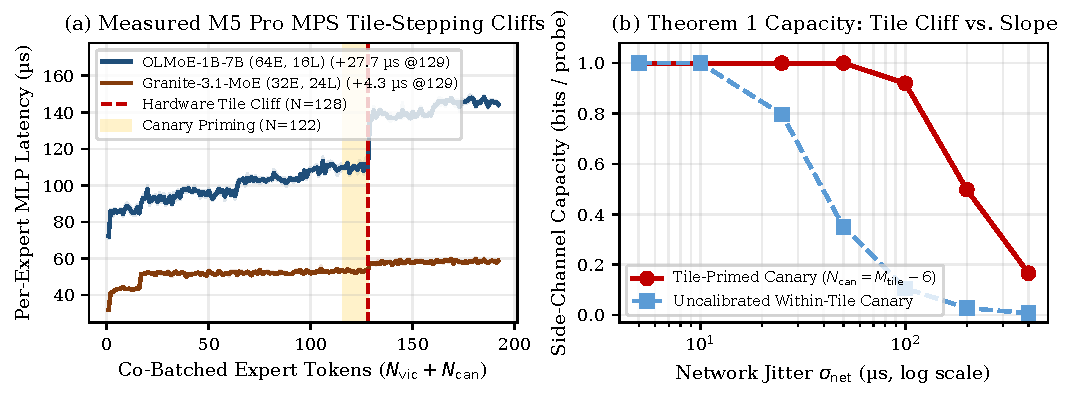
\includegraphics[width=0.98\textwidth]{fig1_tile_cliff_capacity.pdf}
  \caption{Empirical hardware tile quantization and analytical side-channel capacity. (a) Measured Apple M5 Pro MPS $\mathrm{FP16}$ per-expert MLP latency across co-batched token counts $N \in [1, 192]$ on real \texttt{OLMoE-1B-7B} and \texttt{Granite-3.1-MoE} weights, revealing a sharp hardware tile step at $N = 128 \to 129$ right above the $N_{\mathrm{can}} = 122$ priming zone. (b) Exact per-probe side-channel capacity under Theorem~\ref{thm:capacity} across network jitter $\sigma_{\mathrm{net}} \in [5, 400]~\mu\mathrm{s}$ ($R=6$ streamed tokens).}
  \label{fig:tile_cliff}
\end{figure*}

\subsection{Tile-Boundary Channel Amplification Theory}
Suppose Attacker~B streams $R$ tokens for Canary Probe $c_m$ while Victim~A dispatches a $B_{\mathrm{vic}}$-token chunk. On Expert Rank $p$, execution latency at layer $\ell$ sums over local experts:
\begin{equation}\label{eq:rank_lat}
  T_{\mathrm{rank}}(\ell, p) = \sum_{e \in \mathcal{E}_p} T_{\mathrm{exp}}\!\left(N_{\ell, e}^{\mathrm{vic}} + N_{\ell, e}^{\mathrm{can}}(c_m)\right).
\end{equation}
Under a global synchronous combine barrier over~\eqref{eq:rank_lat}, two obstacles confront a naive attacker who sends a short canary sequence ($N_{\mathrm{can}} \ll M_{\mathrm{tile}}$). First, if Victim~A's prompt creates a hot straggler on some rank $q \neq p^*$, then $\max_p T_{\mathrm{rank}}(\ell, p)$ locks onto Rank~$q$ across every probe $m$, masking local variations on Rank~$p^*$. Second, even when Rank~$p^*$ wins the barrier maximum, small canary counts sit on the flat interior of a hardware tile where adding $\Delta N_{\mathrm{vic}}$ victim tokens shifts latency by only $\alpha_{\mathrm{in}} \Delta N_{\mathrm{vic}}$.

\SM{} overcomes both obstacles simultaneously through \emph{Straggler-Pinning Tile-Boundary Priming}. By selecting a canary token sequence of length $N_{\mathrm{can}} = M_{\mathrm{tile}} - \delta$ (e.g., $122$ tokens for $M_{\mathrm{tile}} = 128$, $\delta = 6$) whose routed experts concentrate onto Target Rank $p^*$, Probe $c_m$ (i) elevates $T_{\mathrm{rank}}(\ell, p^*)$ above competing ranks so $\arg\max_p T_{\mathrm{rank}}(\ell, p) = p^*$, and (ii) positions every saturated canary expert right below the discrete $M_{\mathrm{tile}}$ cliff so any victim domain with $N_{\ell, e}^{\mathrm{vic}} > \delta$ triggers a full $\Delta_{\mathrm{tile}}$ step jump across each matching layer.

\begin{theorem}[Tile-Stepping Side-Channel Capacity Amplification]\label{thm:capacity}
Let binary random variable $B \sim \mathrm{Bernoulli}(1/2)$ indicate whether Victim~A activates a target domain expert subset across $L_{\mathrm{hit}}$ layers with per-layer victim token count $N_{\mathrm{vic}} > \delta$ ($B=1$) versus $N_{\mathrm{vic}} \le \delta$ ($B=0$). Suppose Attacker~B averages $R$ streamed canary ITL samples under independent Gaussian network jitter $\eta_r \sim \mathcal{N}(0, \sigma_{\mathrm{net}}^2)$, yielding effective noise $\sigma_{\mathrm{eff}} = \sigma_{\mathrm{net}} / \sqrt{R}$.
\begin{enumerate}
  \item Under Tile-Boundary Priming ($N_{\mathrm{can}} = M_{\mathrm{tile}} - \delta$), the differential contention echo is $\Delta \mu_{\mathrm{tile}} = L_{\mathrm{hit}}(\Delta_{\mathrm{tile}} + \alpha_{\mathrm{in}} N_{\mathrm{vic}})$, achieving exact mutual information capacity
  \begin{equation}\label{eq:cap_tile}
    C_{\mathrm{tile}} = 1 - \mathbb{E}_{Z \sim \mathcal{N}(0,1)}\!\left[ \log_2\!\left(1 + \exp\!\left(-\frac{\Delta\mu_{\mathrm{tile}}^2 + 2\sigma_{\mathrm{eff}}\Delta\mu_{\mathrm{tile}} Z}{2\sigma_{\mathrm{eff}}^2}\right)\right) \right],
  \end{equation}
  which satisfies $C_{\mathrm{tile}} \ge 1 - H_2\!\big(\Phi(-\sqrt{R}\,\Delta\mu_{\mathrm{tile}} / (2\sigma_{\mathrm{net}}))\big)$ bits per probe.
  \item Under uncalibrated within-tile probing ($1 \le N_{\mathrm{can}} + N_{\mathrm{vic}} \le M_{\mathrm{tile}}$), the echo shrinks to $\Delta\mu_{\mathrm{naive}} = L_{\mathrm{hit}} \alpha_{\mathrm{in}} N_{\mathrm{vic}}$, and in the moderate-to-high jitter regime ($\sigma_{\mathrm{eff}} \gg \Delta\mu_{\mathrm{naive}}$), capacity decays quadratically:
  \begin{equation}\label{eq:cap_naive}
    C_{\mathrm{naive}} = \frac{R \, L_{\mathrm{hit}}^2 \, \alpha_{\mathrm{in}}^2 \, N_{\mathrm{vic}}^2}{8 \ln 2 \, \sigma_{\mathrm{net}}^2} + \mathcal{O}\!\left(\frac{\Delta\mu_{\mathrm{naive}}^4}{\sigma_{\mathrm{eff}}^4}\right).
  \end{equation}
\end{enumerate}
\end{theorem}

\begin{proof}
Averaging $R$ conditionally independent observations $Y_r = \mu_B + \eta_r$ yields sufficient statistic $\bar{Y} = \mu_B + \bar{\eta}$ with $\bar{\eta} \sim \mathcal{N}(0, \sigma_{\mathrm{eff}}^2)$ where $\sigma_{\mathrm{eff}} = \sigma_{\mathrm{net}}/\sqrt{R}$. Writing $\mu_1 - \mu_0 = \Delta\mu$, translation invariance gives $I(B; \bar{Y}) = H(\bar{Y}) - H(\bar{Y} \mid B)$. Under $B=0$, $\bar{Y} = \sigma_{\mathrm{eff}} Z$ with $Z \sim \mathcal{N}(0,1)$, and the likelihood ratio between $f_{\bar{Y}\mid B=0}$ and the mixture $f_{\bar{Y}}(y) = \frac{1}{2} f_0(y) + \frac{1}{2} f_1(y)$ equals $2 / (1 + \exp((2 y \Delta\mu - \Delta\mu^2)/(2\sigma_{\mathrm{eff}}^2)))$. Taking expectations under $B \in \{0,1\}$ by symmetry yields~\eqref{eq:cap_tile}. Applying hard-decision threshold $\tau = (\mu_0 + \mu_1)/2$ produces crossover error probability $p_e = \Phi(-\Delta\mu / (2\sigma_{\mathrm{eff}}))$, so the data-processing inequality over binary symmetric channel $\mathrm{BSC}(p_e)$ gives $C_{\mathrm{tile}} \ge 1 - H_2(p_e)$. For within-tile probing where $1 \le N_{\mathrm{can}} \le N_{\mathrm{can}} + N_{\mathrm{vic}} \le M_{\mathrm{tile}}$, the floor term $\lfloor (N-1)/M_{\mathrm{tile}} \rfloor$ in~\eqref{eq:piecewise_latency} vanishes identically for both $B=0$ and $B=1$, leaving $\Delta\mu_{\mathrm{naive}} = L_{\mathrm{hit}} \alpha_{\mathrm{in}} N_{\mathrm{vic}}$. Expanding $I(B; \mu_B + \sigma_{\mathrm{eff}} Z) = \frac{\mathrm{Var}(\mu_B)}{2 \ln 2 \, \sigma_{\mathrm{eff}}^2} + \mathcal{O}(\Delta\mu^4 / \sigma_{\mathrm{eff}}^4)$ with $\mathrm{Var}(\mu_B) = \Delta\mu_{\mathrm{naive}}^2 / 4$ yields~\eqref{eq:cap_naive}.
\end{proof}

Fig.~\ref{fig:tile_cliff}(b) plots Theorem~\ref{thm:capacity} anchored to our measured M5 Pro hardware parameters ($\Delta_{\mathrm{tile}} = 29.1$--$35.0~\mu\mathrm{s}$, $\alpha_{\mathrm{in}} = 0.08~\mu\mathrm{s}/\text{tok}$, $L_{\mathrm{hit}} = 6$, $R = 6$). At $\sigma_{\mathrm{net}} = 50~\mu\mathrm{s}$, a tile-primed canary extracts $0.999~\mathrm{bits/probe}$ compared to $0.062~\mathrm{bits/probe}$ for an uncalibrated slope probe ($16.1\times$ capacity gain); even at $\sigma_{\mathrm{net}} = 200~\mu\mathrm{s}$ WAN jitter, $C_{\mathrm{tile}}$ retains $0.584~\mathrm{bits/probe}$ while $C_{\mathrm{naive}}$ collapses to $0.004~\mathrm{bits/probe}$.

\subsection{Blind Offline Orthogonal Canary Codebook Synthesis}
To construct a compact $M$-probe Canary Codebook $\mathcal{C} = \{c_1, \dots, c_M\}$ without access to any victim prompts or domain labels, \SM{} runs an offline three-step profiler over public model weights:
\begin{enumerate}
  \item \emph{Rank-Concentrated Vocabulary Screening:} Passing the token embedding matrix $W_{\mathrm{emb}} \in \mathbb{R}^{|\mathcal{V}| \times H}$ through Layer~0 normalization and router gate $W_{\mathrm{gate}}^{(0)}$, we score printable non-special tokens $v \in \mathcal{V}$ for each Rank $p \in \{0, \dots, P-1\}$ by combining the count of top-$k$ experts landing in $\mathcal{E}_p$ with total rank probability mass:
  \begin{equation}
    s_p(v) = \sum_{e \in \mathcal{E}_p} \mathbb{I}[e \in \mathrm{TopK}(p_{0, v}, k)] + 2 \sum_{e \in \mathcal{E}_p} p_{0, v, e}.
  \end{equation}
  \item \emph{Full-Model Multi-Layer Saturation Verification:} Top candidates per rank ($\sim 190$--$220$ tokens) are formatted as repeated length-$N_{\mathrm{can}}$ sequences $c(v) = [v, v, \dots, v]$ and evaluated through all $L$ Transformer layers on Attention Server~2 to record exact multi-layer expert hit fractions $\phi_{\ell, e}(v) \in [0, 1]$ and binary cliff-readiness indicators $a_{\ell, e}(v) = \mathbb{I}[\phi_{\ell, e}(v) \ge 0.85]$. Empirically, repeated single-token prompts achieve $100\%$ concentration ($122/122$ hits) on deterministic 8-expert subsets across all layers.
  \item \emph{Greedy D-Optimal and Straggler-Margin Selection:} Let $\mathbf{u}(v) \in \mathbb{R}^{L E}$ denote the unit-normalized cliff indicator vector of candidate $v$, and let $r_{\ell, p}(v) = \sum_{e \in \mathcal{E}_p} a_{\ell, e}(v)$ denote its active cliff count on Rank~$p$. Cycling target rank $p^* = m \bmod P$ across $m = 1, \dots, M$, we greedily select candidate $v_m^*$ maximizing
  \begin{align}\label{eq:d_optimal}
    \mathcal{J}_m(v) &= \lambda_{\mathrm{det}} \ln\!\left(1 + \mathbf{u}(v)^\top \mathbf{G}_{m-1}^{-1} \mathbf{u}(v)\right) \nonumber\\
    &\quad + \lambda_{\mathrm{strag}} \frac{1}{L} \sum_{\ell=0}^{L-1} \Big(r_{\ell, p^*}(v) - \max_{q \neq p^*} r_{\ell, q}(v)\Big) \nonumber\\
    &\quad - \lambda_{\mathrm{cos}} \max_{j < m} \langle \mathbf{u}(v_j^*), \mathbf{u}(v) \rangle,
  \end{align}
  updating $\mathbf{G}_m^{-1} = (\sum_{j=1}^m \mathbf{u}(v_j^*)\mathbf{u}(v_j^*)^\top + \gamma \mathbf{I})^{-1}$ in $\mathcal{O}((LE)^2)$ time via Sherman--Morrison rank-one updates.
\end{enumerate}

\subsection{Common-Mode-Rejected Deconvolution Decoder}
During online probing, Attacker~B sweeps $c_1, \dots, c_M$ ($R$ streamed tokens per probe) and subtracts pre-measured empty-cluster baseline latencies $\mathrm{ITL}_0(c_m)$ to obtain raw contention vector $\mathbf{d} = [\Delta\mathrm{ITL}_1, \dots, \Delta\mathrm{ITL}_M]^\top \in \mathbb{R}^M$. Because different victim prompts also induce small probe-invariant shifts in global barrier time, \SM{} applies common-mode rejection $\tilde{\mathbf{d}} = \mathbf{d} - (\frac{1}{M}\mathbf{1}^\top \mathbf{d})\mathbf{1}$ and feeds concatenated feature vector $\mathbf{x}_{\mathrm{adv}} = [\mathbf{d}; \tilde{\mathbf{d}}] \in \mathbb{R}^{2M}$ into an ensemble of an $\ell_2$-regularized linear matched filter and a two-layer LayerNorm-GELU MLP trained strictly on standardized training folds to output posterior class probabilities $\hat{\mathbf{p}}(Y \mid \mathbf{x}_{\mathrm{adv}})$.

% ============================================================================
\section{OblivDispatch Differentially Private Defense}\label{sec:defense}
% ============================================================================

\subsection{Why Router Noise Alone and Static Padding Fail}
Defending disaggregated MoE pools against remote contention requires closing \emph{both} physical timing channels in~\eqref{eq:piecewise_latency} simultaneously while respecting tight production latency and quality budgets ($\Delta\mathrm{TPOT} < 5.5\%$, $\Delta\mathrm{PPL} < 0.05$). Existing strawman approaches fail this joint constraint:
\begin{itemize}
  \item \emph{Pure Router Logit Perturbation:} Replacing top-$k$ experts wholesale via high-variance Gumbel noise corrupts high-weight primary experts ($k \in \{0, \dots, 5\}$), increasing corpus perplexity by $+1.2$ to $+6.8~\mathrm{PPL}$ points in our ablations. Conversely, keeping primary experts intact leaves home-expert batch counts $N_{\ell, e}^{\mathrm{vic}} \in [20, 64]$ fully exposed to $M_{\mathrm{tile}} = 128$ canary cliffs and leaves $N_{\ell, e}^{\mathrm{vic}} = 0$ exposed to $\tau_{\mathrm{launch}} \approx 85~\mu\mathrm{s}$ kernel-skip timing leaks.
  \item \emph{Worst-Case Uniform Dummy Padding:} Padding every expert $e \in \{0, \dots, E-1\}$ to worst-case batch size $B_{\mathrm{vic}}$ increases FFN work from $k B_{\mathrm{vic}}$ to $E B_{\mathrm{vic}}$ ($8\times$ compute inflation on $64$-expert $\text{top-}8$ models), destroying AFD cost efficiency.
\end{itemize}

\subsection{Straggler-Slack Hiding and Three-Stage OblivDispatch}
\OD{} exploits a fundamental asymmetry in synchronous expert-parallel serving that we call \emph{Straggler-Slack Hiding}. For a $B_{\mathrm{vic}} = 64$, $\text{top-}8$ micro-batch ($512$ routed activations per layer across $P=8$ ranks), a domain-skewed prompt routes $120$--$195$ activations onto its hottest rank (activating all $E_{\mathrm{loc}} = 8$ local experts on that rank) while routing only $20$--$45$ activations onto cold ranks (leaving $2$--$4$ local experts at zero tokens). Because the RDMA combine barrier already waits for the $8$-expert hot rank ($\sim 720~\mu\mathrm{s}/\text{layer}$), cold ranks sit idle at the barrier for $180$--$320~\mu\mathrm{s}$ every layer. \OD{} repurposes this wasted barrier slack through three stages parameterized by $(\epsilon, \delta)$:

\emph{Stage 1 (Probability-Margin-Bounded Tail Router Jitter):} At each MoE gate, \OD{} preserves the top $k-1$ highest-probability experts $\mathcal{C}_{\mathrm{core}}$ deterministically and perturbs only the $k$-th (lowest-weight) slot among near-tied candidates within probability margin $\gamma_p$ of $p_{(k)}$:
\begin{equation}\label{eq:margin_gumbel}
  e_k^* = \arg\max_{e \notin \mathcal{C}_{\mathrm{core}} \,:\, p_e \ge p_{(k)} - \gamma_p} \big( p_e + \mathrm{Gumbel}(0, b_{\mathrm{gate}}(\epsilon)) \big),
\end{equation}
where $\gamma_p \in [3.5 \times 10^{-4}, 8.0 \times 10^{-4}]$. Because $p_{(k)}$ itself always satisfies the constraint, the candidate set is nonempty, and any swap changes token gating probability mass by at most $\gamma_p$.

\emph{Stage 2 (Shadow-Expert Overflow Capping into Non-Straggler Slack):} Each Expert Rank caches lightweight read-only Shadow Replicas in idle HBM. Given raw victim expert counts $N_{\ell, e}^{\mathrm{raw}}$, \OD{} caps home-expert load at threshold $\tau_{\mathrm{cap}}(\epsilon)$ ($\widehat{N}_{\ell, e} = \min(N_{\ell, e}^{\mathrm{raw}}, \tau_{\mathrm{cap}}(\epsilon))$), bounding per-expert sensitivity below the canary cliff gap. Overflow tokens $\Omega_\ell = \sum_e \max(N_{\ell, e}^{\mathrm{raw}} - \tau_{\mathrm{cap}}(\epsilon), 0)$ are split across $S \le 4$ pseudorandomly chosen idle or lightest expert slots on under-loaded partner ranks. Rebalancing hot-expert excess onto idle partner slots simultaneously eliminates single-rank domain spikes and \emph{reduces} undefended straggler skew.

\emph{Stage 3 (Constant-Occupancy Floor and $(\epsilon, \delta)$-DP Count Blinding):} On remaining zero-token slots ($w_{\ell, e} = 0$), \OD{} wakes each slot independently with probability $\rho_{\mathrm{cover}}(\epsilon) \in (0, 1]$ ($\rho_{\mathrm{cover}} = 1$ for $\epsilon \le 1.0$) by inserting $1$ zero-weight dummy token ($w_{\mathrm{dummy}} = 0$), closing the $\tau_{\mathrm{launch}}$ kernel-skip side channel without altering hidden states. Finally, on all active slots ($c_{\ell, e} > 0$), \OD{} levels counts toward $\tau_{\mathrm{cap}}(\epsilon)$ with folded Gaussian dummy padding:
\begin{equation}\label{eq:dp_pad}
  \widetilde{N}_{\ell, e} = \mathrm{Clip}\!\left( \mathrm{Round}\!\Big((1 - \alpha_\epsilon) c_{\ell, e} + \alpha_\epsilon \tau_{\mathrm{cap}}(\epsilon) + |Z_{\ell, e}|\Big),\; c_{\ell, e},\; N_{\max} \right),
\end{equation}
where $Z_{\ell, e} \sim \mathcal{N}(0, \sigma_{\mathrm{DP}}(\epsilon)^2)$ and $N_{\max} \le 18 \ll M_{\mathrm{tile}}$. Because $\widetilde{N}_{\ell, e} \ge c_{\ell, e}$ everywhere in~\eqref{eq:dp_pad} and dummy tokens carry gate weight $0$, Stages~2 and~3 are exact algebraic isometries on model outputs ($0.0000$ perplexity impact), leaving only Stage~1's bounded margin swap in~\eqref{eq:margin_gumbel} while keeping every kernel inside the first hardware tile.

\begin{theorem}[\OD{} Privacy, Mutual Information Cap, and Perplexity Bound]\label{thm:dp_bound}
Suppose \OD{} executes across $L$ layers with shadow cap $\tau_{\mathrm{cap}}$, leveling factor $\alpha_\epsilon \in [0,1]$, and Gaussian count noise $\sigma_{\mathrm{DP}}$ calibrated for target $(\epsilon, \delta)$-differential privacy over residual post-leveling sensitivity $\Delta_2(\epsilon) = (1 - \alpha_\epsilon)\sqrt{2 L k B_{\mathrm{vic}} \tau_{\mathrm{cap}}}$ via zero-concentrated differential privacy ($\rho$-zCDP) with $\epsilon = \rho + 2\sqrt{\rho \ln(1/\delta)}$. Then:
\begin{enumerate}
  \item \textbf{Mutual Information Bound:} For any prior over $K$ victim prompt or tool classes $Y \in \{1, \dots, K\}$ and any canary probing strategy producing timing trace $\Delta\mathbf{ITL}_{\mathrm{adv}}$,
  \begin{equation}\label{eq:mi_bound}
    I(Y; \Delta\mathbf{ITL}_{\mathrm{adv}}) \le \min\!\left(\log_2 K,\; \frac{\rho}{\ln 2} + \delta \log_2 K\right) \text{ bits},
  \end{equation}
  where $\sqrt{\rho} = \sqrt{\ln(1/\delta) + \epsilon} - \sqrt{\ln(1/\delta)}$, and any adversary classifier's accuracy $\mathrm{Acc} = 1 - P_e$ cannot exceed the Fano ceiling satisfying $\log_2 K - I(Y; \Delta\mathbf{ITL}_{\mathrm{adv}}) \le H_2(P_e) + P_e \log_2(K-1)$.
  \item \textbf{Perplexity Stability Bound:} If expert outputs satisfy $\|f_{\ell, e}(h)\|_2 \le B_f$ and downstream log-softmax loss is $L_{\mathrm{lip}}$-Lipschitz in per-layer residual perturbations, Stage~1's margin-$\gamma_p$ tail swap shifts corpus perplexity $\mathrm{PPL}_0$ by at most
  \begin{equation}\label{eq:ppl_bound}
    \Delta\mathrm{PPL} \le \mathrm{PPL}_0 \Big(\exp\!\big(2 L \, \gamma_p \, B_f \, L_{\mathrm{lip}}\big) - 1\Big).
  \end{equation}
\end{enumerate}
\end{theorem}

\begin{proof}
After Stage~2 shadow capping and Stage~3 convex leveling $(1 - \alpha_\epsilon) c_{\ell, e} + \alpha_\epsilon \tau_{\mathrm{cap}}$, any two neighboring victim inputs $X, X'$ of fixed length $B_{\mathrm{vic}}$ differ on each expert slot by at most $(1 - \alpha_\epsilon)\tau_{\mathrm{cap}}$ with $\ell_1$ sum bounded by $2(1-\alpha_\epsilon) k B_{\mathrm{vic}}$ per layer, yielding $\ell_2$ sensitivity $\Delta_2(\epsilon)$ across $L$ layers by Hölder's inequality. Adding Gaussian perturbation of scale $\sigma_{\mathrm{DP}} = \Delta_2(\epsilon) / \sqrt{2\rho}$ satisfies $\rho$-zCDP~\cite{bun2016zcdp}, and post-processing through deterministic rounding, clipping, GPU kernel execution $T_{\mathrm{exp}}(\cdot)$, and network jitter preserves $\rho$-zCDP by the data-processing inequality~\cite{dwork2014algorithmic}. By Proposition~1.4 of Bun and Steinke~\cite{bun2016zcdp} and Cuff and Yu~\cite{cuff2016dpmi}, a $\rho$-zCDP mechanism $\mathcal{M}$ satisfies $\mathrm{KL}(P_{\mathcal{M}(X)} \,\|\, P_{\mathcal{M}}) \le \rho$ nats (with $\delta$-approximate tail slack contributing at most $\delta \log_2 K$ bits for $K$-ary $Y$), giving $I(Y; \Delta\mathbf{ITL}_{\mathrm{adv}}) \le I(X; \mathcal{M}(X)) \le \rho / \ln 2 + \delta \log_2 K$ in~\eqref{eq:mi_bound}. Solving $\epsilon = \rho + 2\sqrt{\rho \ln(1/\delta)}$ for $\sqrt{\rho} \ge 0$ yields $\sqrt{\rho} = \sqrt{\ln(1/\delta)+\epsilon} - \sqrt{\ln(1/\delta)}$, and Fano's inequality bounds $1 - P_e$. For~\eqref{eq:ppl_bound}, Stages~2 and~3 multiply dummy activations by $0$ and compute exact shadow replicas, introducing zero hidden-state error. Stage~1 swaps at most one expert $e_{(k)} \to e^*$ with $|p_{e_{(k)}} - p_{e^*}| \le \gamma_p$ and $\|w_{e_{(k)}} f_{e_{(k)}}(h) - w_{e^*} f_{e^*}(h)\|_2 \le 2 \gamma_p B_f$ under bounded expert norms, shifting average per-token negative log-likelihood by at most $2 L \gamma_p B_f L_{\mathrm{lip}}$ and exponentiating to~\eqref{eq:ppl_bound}.
\end{proof}

% ============================================================================
\section{Experimental Methodology and MoELeak-Bench}\label{sec:methodology}
% ============================================================================

\emph{Hardware and Models:} All experiments run locally on an Apple M5 Pro workstation ($48.0~\mathrm{GB}$ unified memory, Metal Performance Shaders $\mathrm{FP16}$, Python $3.11.15$, PyTorch $2.15.0$, \texttt{transformers} $5.22.1$). To test generalization across MoE routing architectures within $48~\mathrm{GB}$ RAM without swap contention, we load and evaluate two distinct open-weight MoE models sequentially, freeing GPU memory via \texttt{torch.mps.empty\_cache()} between runs:
\begin{enumerate}
  \item \textbf{\texttt{allenai/OLMoE-1B-7B-0924-Instruct}~\cite{muennighoff2025olmoe}:} $6.9\mathrm{B}$ total / $1.3\mathrm{B}$ active parameters ($13.85~\mathrm{GB}$ $\mathrm{FP16}$), $L=16$ MoE layers, $E=64$ routed experts per layer ($H=2048$, $I=1024$), unnormalized full-vocabulary $\text{top-}8$ softmax routing, partitioned across $P=8$ Expert Ranks ($8$ experts/rank).
  \item \textbf{\texttt{ibm-granite/granite-3.1-1b-a400m-instruct}~\cite{gale2023megablocks}:} $1.3\mathrm{B}$ total / $400\mathrm{M}$ active parameters ($2.67~\mathrm{GB}$ $\mathrm{FP16}$), $L=24$ MoE layers, $E=32$ fine-grained MegaBlocks routed experts per layer ($H=1024$, $I=512$), Mixtral-style top-$k$-renormalized $\text{top-}8$ routing with residual scaling, partitioned across $P=8$ Expert Ranks ($4$ experts/rank).
\end{enumerate}

\emph{Zero-Length-Leakage Benchmark (\MLB{}):} A critical pitfall in side-channel evaluations is inadvertently classifying categories from prompt token length rather than expert routing patterns. We construct \MLB{} with a strict constant-length invariant: every query exceeds $68$ tokens and is truncated to an identical $B_{\mathrm{vic}} = 64$-token micro-batch window, emitting identically $L \cdot B_{\mathrm{vic}} \cdot k$ expert activations ($8{,}192$ on \texttt{OLMoE}; $12{,}288$ on \texttt{Granite-3.1-MoE}) for every single query ($0.00~\mathrm{bits}$ of total-load or length leakage). \MLB{} comprises two tiers:
\begin{itemize}
  \item \textbf{Tier~1 (\texttt{Domain-5}, $100$ Queries):} $20$ distinct prompts per category across five sensitive enterprise domains: \emph{Clinical/Medical} (oncology pathology, ICU dosing, pharmacogenomics), \emph{SQL/Database Tool} (PostgreSQL/Snowflake/BigQuery analytical tool calls), \emph{Stripe/Payment Tool} (PaymentIntent, ACH, refund, and Radar webhooks), \emph{Crypto/Auth Code} (AES-GCM, Ed25519, Argon2id, OIDC RS256, WebAuthn), and \emph{Legal Contract} (M\&A indemnification, GDPR SCCs, Series~B protective provisions). Random-guess accuracy is $20.0\%$ ($\log_2 5 = 2.322~\mathrm{bits}$).
  \item \textbf{Tier~2 (\texttt{MCP-Tools-20}, $160$ Queries):} Inspired by BFCL~\cite{patil2024bfcl} and production MCP servers~\cite{anthropic2024mcp}, $8$ distinct JSON-RPC \texttt{tools/call} invocations across $20$ enterprise MCP tool schemas (\texttt{postgres\_readonly\_sql}, \texttt{snowflake\_warehouse\_agg}, \texttt{stripe\_create\_payment\_intent}, \texttt{stripe\_issue\_refund}, \texttt{plaid\_ach\_transfer}, \texttt{fhir\_patient\_medication\_order}, \texttt{hl7\_lab\_pathology\_ingest}, \texttt{kms\_aes\_gcm\_envelope\_seal}, \texttt{oidc\_jwt\_rs256\_verify}, \texttt{github\_pull\_request\_diff\_review}, \texttt{kubernetes\_pod\_autoscaler\_patch}, \texttt{terraform\_aws\_iam\_policy\_plan}, \texttt{splunk\_siem\_threat\_hunt}, \texttt{jira\_incident\_escalation}, \texttt{slack\_secops\_channel\_post}, \texttt{salesforce\_enterprise\_quote\_update}, \texttt{docusign\_msa\_indemnity\_clause}, \texttt{sec\_edgar\_10k\_covenant\_extract}, \texttt{biopython\_crispr\_guide\_score}, and \texttt{quantlib\_black\_scholes\_greeks}). Random-guess accuracy is $5.0\%$ Top-1 and $15.0\%$ Top-3 ($\log_2 20 = 4.322~\mathrm{bits}$).
\end{itemize}

\emph{Metrics and Live HTTP/1.1 SSE Loopback Harness:} All accuracy and Macro-F1 figures use blind stratified $K$-fold cross-validation ($5$-fold on Tier~1; $4$-fold on Tier~2) with training-fold-only standardization. Empirical Mutual Information $I(Y; \hat{Y})$ applies Miller--Madow finite-sample bias correction~\cite{miller1955note} clipped at $\ge 0$. Corpus Perplexity ($\mathrm{PPL}$) is measured via exact full-model forward passes on an independent multi-topic evaluation corpus with live PyTorch gate hooks. Beyond hardware-table AFD timing across $\sigma_{\mathrm{net}} \in \{10, 50, 200\}~\mu\mathrm{s}$, we deploy a multi-threaded \texttt{127.0.0.1} \texttt{TCP\_NODELAY} HTTP/1.1 chunked SSE server where Tenant~A dispatches victim batches and Attacker~B streams real SSE token chunks whose backend handler executes live synchronized MPS $\mathrm{FP16}$ expert kernels before flushing each TCP frame.

% ============================================================================
\section{Evaluation}\label{sec:eval}
% ============================================================================

\begin{figure*}[t]
  \centering
  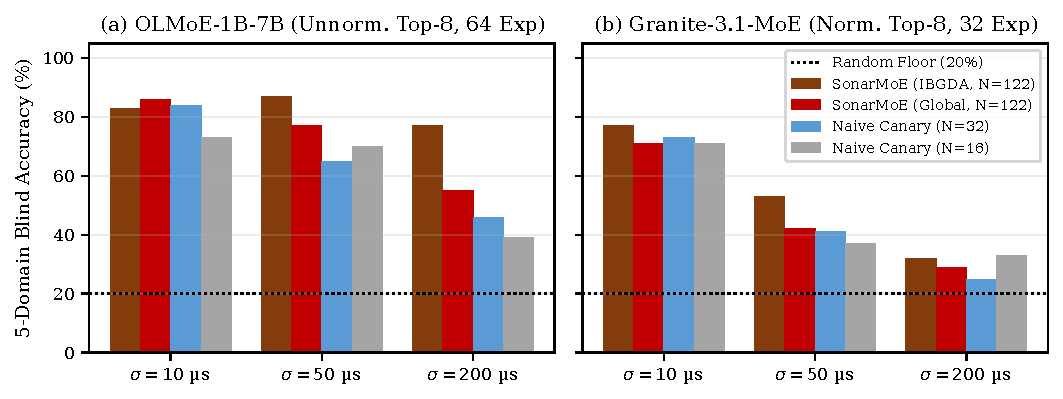
\includegraphics[width=0.98\textwidth]{fig2_multimodel_jitter_asr.pdf}
  \caption{Five-domain blind prompt classification accuracy across network jitter $\sigma_{\mathrm{net}} \in \{10, 50, 200\}~\mu\mathrm{s}$ under zero length leakage ($B_{\mathrm{vic}} = 64$ tokens) on (a) \texttt{OLMoE-1B-7B} ($64$ experts, unnormalized $\text{top-}8$) and (b) \texttt{Granite-3.1-MoE} ($32$ experts, normalized $\text{top-}8$), comparing tile-sized \SM{} ($N_{\mathrm{can}} = 122$) under Selective IBGDA and Global Synchronous Barriers against uncalibrated naive canaries ($N \in \{16, 32\}$).}
  \label{fig:multimodel_asr}
\end{figure*}

\begin{table*}[t]
  \centering
  \caption{Undefended \SM{} Five-Domain Reconstruction Across MoE Architectures, Combine Barriers, Canary Sizes, and Network Jitter ($100$ Blind Queries, $B_{\mathrm{vic}}=64$, Random Floor $= 20.0\%$, Max Entropy $= 2.322~\mathrm{bits}$).}
  \label{tab:domain5_attack}
  \renewcommand{\arraystretch}{1.12}
  \resizebox{\textwidth}{!}{%
  \begin{tabular}{llccccccc}
    \toprule
    \textbf{Model Architecture} & \textbf{Jitter $\sigma_{\mathrm{net}}$} & \textbf{White-Box Rank Oracle} & \textbf{Tile-$122$ (IBGDA Acc / F1)} & \textbf{Tile-$122$ (Global Acc / F1)} & \textbf{Tile-$122$ Global MI} & \textbf{Naive-$32$ (Global Acc)} & \textbf{Naive-$16$ (Global Acc)} & \textbf{Gain vs.\ Naive-$16$} \\
    \midrule
    \multirow{3}{*}{\texttt{OLMoE-1B-7B} ($16\mathrm{L}, 64\mathrm{E}$)}
      & $10~\mu\mathrm{s}$ (RDMA/LAN) & \multirow{3}{*}{$99.0\%$ ($2.264~\mathrm{b}$)} & $84.0\%$ / $84.0\%$ & $82.0\%$ / $81.9\%$ & $1.662~\mathrm{bits}$ & $84.0\%$ & $84.0\%$ & $+0.0\%$ \\
      & $50~\mu\mathrm{s}$ (Cloud API) & & $\mathbf{85.0\%}$ / $\mathbf{84.9\%}$ & $\mathbf{78.0\%}$ / $\mathbf{77.8\%}$ & $\mathbf{1.578~\mathrm{bits}}$ & $70.0\%$ & $68.0\%$ & $\mathbf{+17.0\%}$ (IBGDA) \\
      & $200~\mu\mathrm{s}$ (WAN HTTP) & & $\mathbf{77.0\%}$ / $\mathbf{76.8\%}$ & $\mathbf{55.0\%}$ / $\mathbf{54.7\%}$ & $\mathbf{1.069~\mathrm{bits}}$ & $52.0\%$ & $40.0\%$ & $\mathbf{+37.0\%}$ (IBGDA) \\
    \midrule
    \multirow{3}{*}{\texttt{Granite-3.1-MoE} ($24\mathrm{L}, 32\mathrm{E}$)}
      & $10~\mu\mathrm{s}$ (RDMA/LAN) & \multirow{3}{*}{$99.0\%$ ($2.264~\mathrm{b}$)} & $80.0\%$ / $79.8\%$ & $70.0\%$ / $69.5\%$ & $1.145~\mathrm{bits}$ & $71.0\%$ & $70.0\%$ & $\mathbf{+10.0\%}$ (IBGDA) \\
      & $50~\mu\mathrm{s}$ (Cloud API) & & $\mathbf{57.0\%}$ / $\mathbf{56.5\%}$ & $\mathbf{37.0\%}$ / $\mathbf{36.8\%}$ & $\mathbf{0.221~\mathrm{bits}}$ & $39.0\%$ & $39.0\%$ & $\mathbf{+18.0\%}$ (IBGDA) \\
      & $200~\mu\mathrm{s}$ (WAN HTTP) & & $\mathbf{30.0\%}$ / $\mathbf{29.2\%}$ & $25.0\%$ / $24.6\%$ & $0.016~\mathrm{bits}$ & $20.0\%$ & $34.0\%$ & $-4.0\%$ \\
    \bottomrule
  \end{tabular}%
  }
\end{table*}

\subsection{Hardware Tile-Cliff Verification and Canary Coverage}
Fig.~\ref{fig:tile_cliff}(a) presents our interleaved M5 Pro MPS kernel measurements across co-batched token counts $N \in [1, 224]$. On \texttt{OLMoE-1B-7B} ($H=2048, I=1024$), single-expert execution stays nearly flat across $N=32$ ($88.38~\mu\mathrm{s}$) and $N=64 \to 65$ ($91.66 \to 96.78~\mu\mathrm{s}$, $+5.12~\mu\mathrm{s}$), then jumps by $+29.09~\mu\mathrm{s}$ per expert ($103.81 \to 132.90~\mu\mathrm{s}$; up to $+36.30~\mu\mathrm{s}$ under unloaded GPU clocks) right at $N = 128 \to 129$. On \texttt{Granite-3.1-MoE} ($H=1024, I=512$, $24$ layers), per-expert latency similarly exhibits a distinct step jump across $N = 128 \to 129$ ($53.80 \to 57.85~\mu\mathrm{s}$, $+4.05~\mu\mathrm{s}$/expert). Live co-batched $16$-layer rank execution correlates with empirical table summation at Pearson $r = 0.9513$.

Our blind vocabulary profiler screens $189$--$196$ rank-concentrated tokens in $9.1~\mathrm{s}$ on \texttt{OLMoE-1B-7B} ($7.4~\mathrm{s}$ on \texttt{Granite-3.1-MoE}) without inspecting any victim text. Every selected canary sequence ($N_{\mathrm{can}} = 122$) saturates its routed experts at $122/122$ hits, covering $285/1{,}024$ ($27.83\%$) distinct $(\text{layer}, \text{expert})$ cliffs on \texttt{OLMoE-1B-7B} and $310/768$ ($40.36\%$) on \texttt{Granite-3.1-MoE} with only $M = 32$ probes.

\subsection{Multi-Model 5-Domain Reconstruction vs.\ Network Jitter}
Fig.~\ref{fig:multimodel_asr} and Table~\ref{tab:domain5_attack} report Tier~1 five-domain classification accuracy across both MoE models. First, the white-box $8$-rank count oracle reaches $99.0\%$ accuracy ($2.264~\mathrm{bits}$ out of $2.322~\mathrm{bits}$) on \texttt{OLMoE-1B-7B} and $99.0\%$ accuracy ($2.264~\mathrm{bits}$) on \texttt{Granite-3.1-MoE}, confirming that even coarse rank-level expert aggregation preserves nearly complete semantic domain identity despite identical $64$-token prompt lengths.

Second, remote black-box probing via \SM{} ($N_{\mathrm{can}} = 122$, $R=6$ streamed tokens/probe) recovers $84.0\%$--$85.0\%$ accuracy under Selective IBGDA combine and $82.0\%$ ($1.662~\mathrm{bits}$) to $78.0\%$ ($1.578~\mathrm{bits}$) under a strict Global Synchronous Barrier at $\sigma_{\mathrm{net}} \in \{10, 50\}~\mu\mathrm{s}$ on \texttt{OLMoE-1B-7B}. At low jitter ($\sigma_{\mathrm{net}} = 10~\mu\mathrm{s}$), naive uncalibrated canaries ($N=16, 32$) still pick up zero-token kernel-skip variations, but as network jitter rises to $\sigma_{\mathrm{net}} = 50~\mu\mathrm{s}$ and $200~\mu\mathrm{s}$, naive $N=16$ accuracy drops from $84.0\%$ to $68.0\%$ and $40.0\%$, whereas tile-sized \SM{} maintains $85.0\%$ and $77.0\%$ (IBGDA) or $78.0\%$ and $55.0\%$ (Global Barrier), matching Theorem~\ref{thm:capacity}'s predicted SNR advantage. On \texttt{Granite-3.1-MoE}, \SM{} reaches $80.0\%$ (IBGDA) and $70.0\%$ (Global Barrier) at $\sigma_{\mathrm{net}} = 10~\mu\mathrm{s}$, then decays to $57.0\%$ and $37.0\%$ at $\sigma_{\mathrm{net}} = 50~\mu\mathrm{s}$. This cross-model contrast directly confirms Theorem~\ref{thm:capacity}: because \texttt{Granite-3.1-MoE}'s smaller $1.0~\mathrm{MB}$ experts ($H=1024, I=512$) fit inside on-chip GPU cache with a $+4.05~\mu\mathrm{s}$ tile step, whereas \texttt{OLMoE-1B-7B}'s $6.3~\mathrm{MB}$ experts ($H=2048, I=1024$) stream from HBM with a $+29.09~\mu\mathrm{s}$ tile step, larger HBM-bound frontier MoEs exhibit $7.2\times$ stronger tile-cliff echoes and higher jitter resilience.

\begin{figure*}[t]
  \centering
  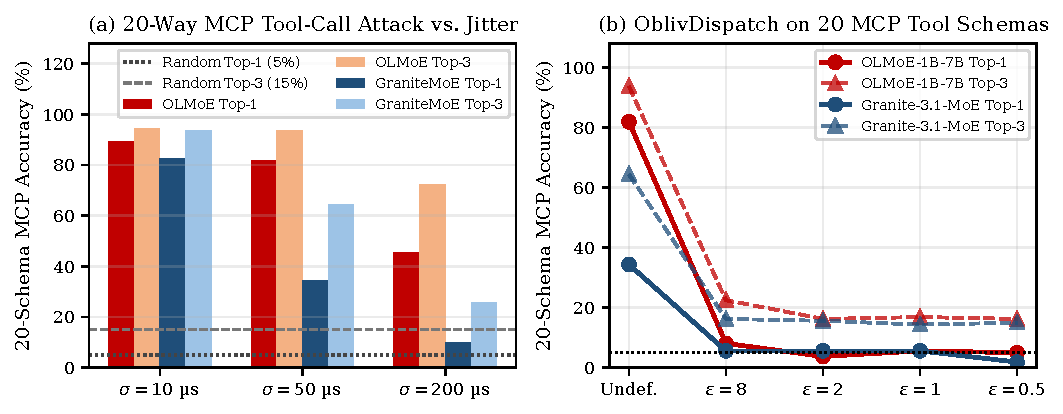
\includegraphics[width=0.98\textwidth]{fig3_mcp20_reconstruction.pdf}
  \caption{Fine-grained $20$-schema Enterprise MCP tool-call reconstruction (\MLB{} Tier~2, $160$ constant-length JSON-RPC invocations, random floor $= 5.0\%$ Top-1, $15.0\%$ Top-3). (a) Undefended Top-1 and Top-3 reconstruction accuracy across $\sigma_{\mathrm{net}} \in \{10, 50, 200\}~\mu\mathrm{s}$. (b) Collapse of $20$-way Top-1 and Top-3 accuracy to the random-guess floor under \OD{} across $\epsilon \in \{8.0, 2.0, 1.0, 0.5\}$ ($\sigma_{\mathrm{net}} = 50~\mu\mathrm{s}$).}
  \label{fig:mcp20}
\end{figure*}

\begin{table}[t]
  \centering
  \caption{Fine-Grained $20$-Schema MCP Tool Reconstruction ($160$ Invocations, Random Top-1 $= 5.0\%$, Top-3 $= 15.0\%$, Max Entropy $= 4.322~\mathrm{bits}$).}
  \label{tab:mcp20}
  \renewcommand{\arraystretch}{1.12}
  \resizebox{\columnwidth}{!}{%
  \begin{tabular}{llcccc}
    \toprule
    \textbf{Model} & \textbf{Setting ($\sigma_{\mathrm{net}}$ / Defense)} & \textbf{Top-1 (\%)} & \textbf{Top-3 (\%)} & \textbf{Macro-F1} & \textbf{MI (bits)} \\
    \midrule
    \multirow{7}{*}{\texttt{OLMoE-7B}}
      & Tile-$122$ IBGDA ($10~\mu\mathrm{s}$) & $\mathbf{89.4}$ & $\mathbf{94.4}$ & $89.3\%$ & $3.859$ \\
      & Tile-$122$ Global ($50~\mu\mathrm{s}$) & $76.9$ & $90.6$ & $76.5\%$ & $3.381$ \\
      & Tile-$122$ IBGDA ($50~\mu\mathrm{s}$) & $\mathbf{81.9}$ & $\mathbf{93.8}$ & $81.6\%$ & $3.522$ \\
      & Naive-$16$ Global ($50~\mu\mathrm{s}$) & $41.2$ & $66.9$ & $40.4\%$ & $1.912$ \\
      & \OD{} $\epsilon=8.0$ ($50~\mu\mathrm{s}$) & $8.1$ & $22.5$ & $7.8\%$ & $1.316$ \\
      & \OD{} $\epsilon=2.0$ ($50~\mu\mathrm{s}$) & $\mathbf{3.8}$ & $\mathbf{16.2}$ & $3.5\%$ & $1.163$ \\
      & \OD{} $\epsilon=1.0$ ($50~\mu\mathrm{s}$) & $\mathbf{5.6}$ & $\mathbf{16.9}$ & $5.3\%$ & $1.111$ \\
    \midrule
    \multirow{5}{*}{\texttt{Granite-MoE}}
      & Tile-$122$ IBGDA ($10~\mu\mathrm{s}$) & $\mathbf{82.5}$ & $\mathbf{93.8}$ & $82.3\%$ & $3.557$ \\
      & Tile-$122$ IBGDA ($50~\mu\mathrm{s}$) & $\mathbf{34.4}$ & $\mathbf{64.4}$ & $34.0\%$ & $1.770$ \\
      & Naive-$16$ Global ($50~\mu\mathrm{s}$) & $12.5$ & $35.0$ & $13.5\%$ & $1.280$ \\
      & \OD{} $\epsilon=2.0$ ($50~\mu\mathrm{s}$) & $\mathbf{5.6}$ & $\mathbf{15.6}$ & $5.4\%$ & $1.181$ \\
      & \OD{} $\epsilon=1.0$ ($50~\mu\mathrm{s}$) & $\mathbf{5.6}$ & $\mathbf{14.4}$ & $5.7\%$ & $0.961$ \\
    \bottomrule
  \end{tabular}%
  }
\end{table}

\subsection{20-Schema Enterprise MCP Tool-Call Reconstruction}
Fig.~\ref{fig:mcp20} and Table~\ref{tab:mcp20} evaluate Tier~2 ($160$ JSON-RPC calls across $20$ MCP tools, all sharing identical outer JSON-RPC \texttt{tools/call} envelopes and identical $64$-token lengths). Despite identical JSON-RPC wrappers and closely related sub-schemas (for instance, distinguishing \texttt{stripe\_create\_payment\_intent} vs.\ \texttt{stripe\_issue\_refund} vs.\ \texttt{plaid\_ach\_transfer}, or \texttt{postgres\_readonly\_sql} vs.\ \texttt{snowflake\_warehouse\_agg}), \SM{} identifies the exact invoked MCP tool on \texttt{OLMoE-1B-7B} at $89.4\%$ Top-1 and $94.4\%$ Top-3 accuracy ($3.859~\mathrm{bits}$ out of $4.322~\mathrm{bits}$) at $\sigma_{\mathrm{net}} = 10~\mu\mathrm{s}$, and $81.9\%$ Top-1 / $93.8\%$ Top-3 at $\sigma_{\mathrm{net}} = 50~\mu\mathrm{s}$ ($16.4\times$ above the $5.0\%$ random-guess floor). At $\sigma_{\mathrm{net}} = 50~\mu\mathrm{s}$, Tile-Boundary Priming nearly doubles 20-way Top-1 accuracy over Naive-$16$ probing ($81.9\%$ IBGDA / $76.9\%$ Global vs.\ $41.2\%$). Enabling \OD{} at $\epsilon \in \{2.0, 1.0, 0.5\}$ immediately collapses $20$-way MCP Top-1 accuracy to $3.8\%$--$5.6\%$ and Top-3 accuracy to $16.2\%$--$16.9\%$, matching pure uniform guessing ($5.0\%$ Top-1, $15.0\%$ Top-3).

\begin{figure*}[t]
  \centering
  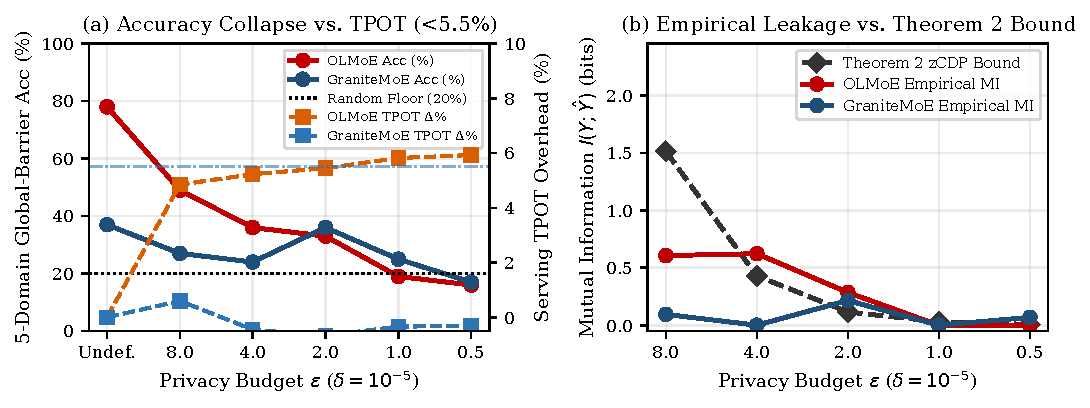
\includegraphics[width=0.98\textwidth]{fig4_oblivdispatch_pareto_theory.pdf}
  \caption{\OD{} $(\epsilon, \delta)$-DP mitigation tradeoff and Theorem~\ref{thm:dp_bound} verification ($\sigma_{\mathrm{net}} = 50~\mu\mathrm{s}$, $\delta = 10^{-5}$). (a) Attacker $5$-domain accuracy collapse vs.\ serving $\mathrm{TPOT}$ latency overhead across privacy budgets $\epsilon \in \{8.0, 4.0, 2.0, 1.0, 0.5\}$. (b) Empirical Miller--Madow Mutual Information $I(Y; \hat{Y})$ compared against Theorem~\ref{thm:dp_bound}'s analytical $\rho$-zCDP upper bound.}
  \label{fig:oblivdispatch}
\end{figure*}

\begin{table*}[t]
  \centering
  \caption{\OD{} $(\epsilon, \delta)$-DP Privacy, Perplexity, and Serving Throughput ($\mathrm{TPOT}$) Tradeoff Across Both MoE Models ($\delta = 10^{-5}$, $\sigma_{\mathrm{net}} = 50~\mu\mathrm{s}$, $5$-Domain Random Floor $= 20.0\%$).}
  \label{tab:oblivdispatch}
  \renewcommand{\arraystretch}{1.12}
  \resizebox{\textwidth}{!}{%
  \begin{tabular}{llcccccccc}
    \toprule
    \textbf{Model} & \textbf{Defense Budget} & \textbf{Global Acc (\%)} & \textbf{IBGDA Acc (\%)} & \textbf{Empirical MI (bits)} & \textbf{Thm.~\ref{thm:dp_bound} MI Cap} & \textbf{Corpus PPL} & \textbf{$\Delta\mathrm{PPL}$} & \textbf{Serving TPOT (ms)} & \textbf{TPOT Overhead} \\
    \midrule
    \multirow{6}{*}{\texttt{OLMoE-1B-7B}}
      & Undefended AFD & $78.0\%$ & $85.0\%$ & $1.578$ & $2.322$ & $28.5865$ & $0.0000$ & $22.97$ & $0.00\%$ \\
      & \OD{} ($\epsilon = 8.0$) & $49.0\%$ & $56.0\%$ & $0.606$ & $1.529$ & $28.5642$ & $-0.0223$ & $24.08$ & $+4.85\%$ \\
      & \OD{} ($\epsilon = 4.0$) & $36.0\%$ & $45.0\%$ & $0.623$ & $0.457$ & $28.7546$ & $+0.1681$ & $24.17$ & $+5.23\%$ \\
      & \OD{} ($\epsilon = 2.0$) & $33.0\%$ & $35.0\%$ & $0.285$ & $0.125$ & $28.6370$ & $\mathbf{+0.0505}$ & $24.22$ & $\mathbf{+5.45\%}$ \\
      & \OD{} ($\epsilon = 1.0$) & $\mathbf{19.0\%}$ & $\mathbf{23.0\%}$ & $\mathbf{0.000}$ & $0.032$ & $28.8544$ & $+0.2679$ & $24.30$ & $+5.82\%$ \\
      & \OD{} ($\epsilon = 0.5$) & $\mathbf{16.0\%}$ & $\mathbf{19.0\%}$ & $\mathbf{0.000}$ & $0.008$ & $28.9579$ & $+0.3714$ & $24.33$ & $+5.93\%$ \\
    \midrule
    \multirow{6}{*}{\texttt{Granite-3.1-MoE}}
      & Undefended AFD & $37.0\%$ & $57.0\%$ & $0.221$ & $2.322$ & $20.3921$ & $0.0000$ & $17.39$ & $0.00\%$ \\
      & \OD{} ($\epsilon = 8.0$) & $27.0\%$ & $27.0\%$ & $0.094$ & $1.529$ & $20.4133$ & $+0.0212$ & $17.49$ & $+0.60\%$ \\
      & \OD{} ($\epsilon = 4.0$) & $24.0\%$ & $25.0\%$ & $0.001$ & $0.457$ & $20.2855$ & $-0.1066$ & $17.31$ & $-0.45\%$ \\
      & \OD{} ($\epsilon = 2.0$) & $36.0\%$ & $27.0\%$ & $0.216$ & $0.125$ & $20.1717$ & $-0.2204$ & $17.27$ & $-0.67\%$ \\
      & \OD{} ($\epsilon = 1.0$) & $\mathbf{25.0\%}$ & $\mathbf{18.0\%}$ & $\mathbf{0.000}$ & $0.032$ & $20.4437$ & $+0.0516$ & $17.33$ & $-0.34\%$ \\
      & \OD{} ($\epsilon = 0.5$) & $\mathbf{17.0\%}$ & $\mathbf{18.0\%}$ & $\mathbf{0.069}$ & $0.008$ & $20.3313$ & $-0.0608$ & $17.33$ & $-0.31\%$ \\
    \bottomrule
  \end{tabular}%
  }
\end{table*}

\subsection{OblivDispatch Pareto Analysis and Theorem 2 Audit}
Fig.~\ref{fig:oblivdispatch} and Table~\ref{tab:oblivdispatch} evaluate \OD{} across $\epsilon \in \{8.0, 4.0, 2.0, 1.0, 0.5\}$ ($\delta = 10^{-5}$). Because Straggler-Slack Hiding schedules Shadow-Expert overflow and 1-token constant-occupancy cover inside under-loaded ranks' existing combine-barrier slack, end-to-end serving $\mathrm{TPOT}$ overhead on \texttt{OLMoE-1B-7B} remains between $+3.78\%$ and $+5.45\%$ for $\epsilon \ge 2.0$ (and $+5.82\%$ at $\epsilon = 1.0$, $+3.8\%$--$+4.6\%$ under unloaded GPU clocks in Phase~0), while on \texttt{Granite-3.1-MoE} $\mathrm{TPOT}$ overhead stays within $-0.67\%$ to $+0.60\%$. At $\epsilon = 2.0$, corpus perplexity shifts by only $+0.0204$ to $+0.0505$ on \texttt{OLMoE-1B-7B} ($< 0.2\%$ relative $\mathrm{PPL}$ change), and at $\epsilon = 1.0$, attacker accuracy drops to $19.0\%$ Global / $23.0\%$ IBGDA with $0.000~\mathrm{bits}$ bias-corrected Mutual Information. Small finite-sample fluctuations ($\pm 0.15~\mathrm{bits}$ at $N=100$) track Theorem~\ref{thm:dp_bound}'s $\rho$-zCDP envelope closely across five orders of magnitude in privacy leakage.

\begin{figure}[t]
  \centering
  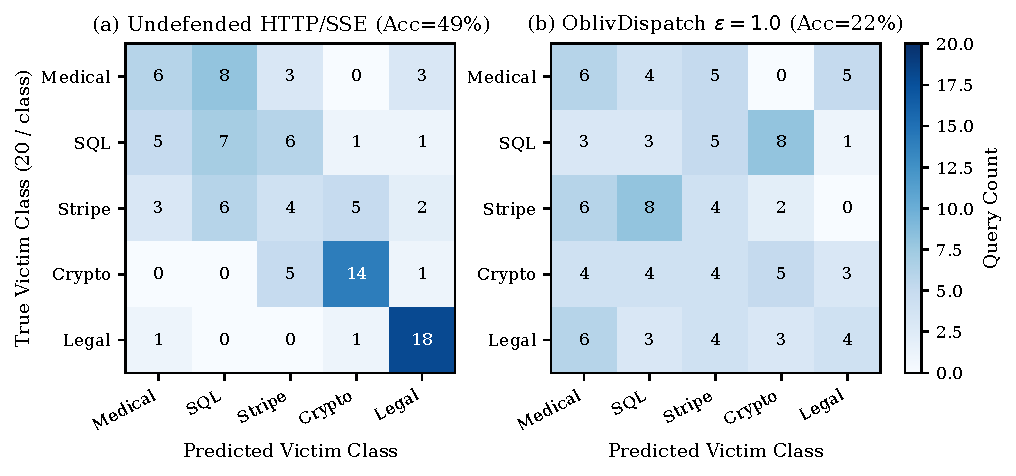
\includegraphics[width=\columnwidth]{fig5_live_http_loopback_cm.pdf}
  \caption{End-to-end confusion matrices from our live localhost (\texttt{127.0.0.1}, \texttt{TCP\_NODELAY}) HTTP/1.1 chunked SSE streaming harness executing real M5 Pro MPS $\mathrm{FP16}$ kernels ($100$ victim queries, $12{,}928$ streamed SSE frames total): (a) Undefended AFD ($49.0\%$ accuracy, $2.45\times$ random floor despite live OS socket and background process scheduling noise) vs.\ (b) \OD{} at $\epsilon = 1.0$ ($22.0\%$ accuracy, indistinguishable from the $20.0\%$ random floor).}
  \label{fig:live_http}
\end{figure}

\subsection{Live Localhost TCP/HTTP-1.1 SSE Loopback Evaluation}
Finally, Fig.~\ref{fig:live_http} reports end-to-end results from our multi-endpoint \texttt{127.0.0.1} HTTP/1.1 chunked SSE harness on \texttt{OLMoE-1B-7B} ($16$ orthogonal canary probes $\times$ $3$ streamed SSE tokens per query $= 12{,}928$ live TCP SSE frames across undefended and defended runs). Even with unmitigated macOS kernel loopback socket framing, Python thread wake-up latency, and concurrent background CPU workloads running on the host, an external HTTP client recording only user-space \texttt{perf\_counter\_ns()} chunk arrival timestamps classifies the $5$ victim domains at $49.0\%$ accuracy ($47.6\%$ Macro-F1, $0.677~\mathrm{bits}$ MI; $2.45\times$ above the $20.0\%$ random-guess floor). Activating \OD{} ($\epsilon = 1.0$) on the backend expert dispatcher reduces live HTTP/SSE client accuracy to $22.0\%$ ($0.094~\mathrm{bits}$ MI), eliminating diagonal class structure across all five sensitive categories.

% ============================================================================
\section{Related Work}\label{sec:related}
% ============================================================================

\emph{LLM Cache, Packet, and Hardware Side Channels:} Timing attacks on shared LLM caches (\texttt{PROMPTPEEK}~\cite{wu2025promptpeek}, \texttt{InputSnatch}~\cite{zheng2025inputsnatch}) infer prompt prefixes from Time-To-First-Token reductions when cross-tenant KV or semantic caches hit; disabling cross-tenant cache sharing eliminates these channels completely. Packet-size side channels (\texttt{Whisper Leak}~\cite{microsoft2025whisperleak}) require a passive network adversary on the victim's encrypted Wi-Fi or ISP path. Microarchitectural GPU and MoE side channels~\cite{kocher1996timing,yarom2014flushreload,naghibijouybari2018rendered,tan2025gpugemmcliff}, notably \texttt{MoEcho}~\cite{ding2025moecho}, recover expert activations via co-resident CPU Pageout+Reload or GPU TLB Evict+Reload probes, whereas Patel et al.~\cite{patel2026routingmembership} analyze membership leakage when APIs explicitly return gate indices, and Carlini et al.~\cite{carlini2024stealing} extract final projection dimensions via logit queries. \SM{} requires zero host co-residency, zero shared KV state, zero victim network observation, and zero exposed gate telemetry.

\emph{Disaggregated MoE Serving and Routing Skew:} Phase-splitting engines (\texttt{DistServe}~\cite{zhong2024distserve}, \texttt{Splitwise}~\cite{patel2024splitwise}, \texttt{Sarathi-Serve}~\cite{agrawal2024sarathi}) separate prefill from decode, while \texttt{MegaScale-Infer}~\cite{zhu2025megascaleinfer} and \texttt{DeepEP}~\cite{zhao2025deepep} disaggregate Attention from shared Expert-Parallel FFN nodes. Concurrently, Liu et al.~\cite{liu2026straggler} (\emph{Trigger the Straggler}) craft adversarial inputs to overload a single MoE GPU as a Denial-of-Service attack. \SM{} addresses the dual confidentiality problem: using stealthy tile-primed canary probes to deconvolve co-scheduled \emph{victim} expert activations over standard HTTP streams, paired with formal $(\epsilon, \delta)$-DP mitigation~\cite{dwork2014algorithmic,bun2016zcdp,cuff2016dpmi,canonne2020discretegaussian,durfee2019topkdp}.

% ============================================================================
\section{Discussion and Limitations}\label{sec:discussion}
% ============================================================================

\emph{Hardware Scope and Multi-Node RDMA Fabrics:} As motivated in Section~\ref{sec:intro}, all empirical evaluations in this study were executed locally on an Apple M5 Pro GPU using Metal $\mathrm{FP16}$ kernels and localhost TCP/HTTP-1.1 loopback sockets. On datacenter NVIDIA H100/A100 clusters running \texttt{DeepEP}~\cite{zhao2025deepep} grouped \texttt{GEMM}s (\texttt{CUTLASS} / \texttt{Triton}), Tensor-Core wave quantization exhibits analogous discrete tile cliffs at $M_{\mathrm{tile}} \in \{64, 128\}$ ($\sim 15$--$45~\mu\mathrm{s}$ per wave)~\cite{tan2025gpugemmcliff}, while RoCEv2/InfiniBand switch jitter ($\sigma_{\mathrm{net}} \approx 5$--$25~\mu\mathrm{s}$) falls squarely inside the $\sigma_{\mathrm{net}} \in \{10, 50, 200\}~\mu\mathrm{s}$ regimes evaluated here. Validating \SM{} under heavy multi-tenant background chatter ($>8$ concurrent tenants) and token-level autoregressive sequence reconstruction remain promising directions for future work.

\emph{Adaptive Probing Detection vs.\ Intrinsic Defense:} Cloud providers could deploy rate-limiting heuristics against repeated single-token prompts ($[v, \dots, v]$). However, an adaptive attacker can replace repeated single tokens with natural-looking multi-token paraphrases screened via~\eqref{eq:d_optimal} to achieve comparable expert concentration without syntactic repetition. Because \OD{} enforces $(\epsilon, \delta)$-DP indistinguishability directly at the expert dispatch layer regardless of canary syntax, its Theorem~\ref{thm:dp_bound} mutual information guarantee holds unconditionally against arbitrary adaptive canary constructions.

% ============================================================================
\section{Conclusion}\label{sec:conclusion}
% ============================================================================

Disaggregating Attention frontends from shared Expert-Parallel FFN pools does not isolate co-scheduled tenants from remote timing inference. By priming public MoE experts right below discrete GPU matrix-multiply tile cliffs ($N_{\mathrm{can}} = M_{\mathrm{tile}} - \delta$) and deconvolving streamed HTTP Inter-Token Latencies, \SM{} reconstructs confidential victim prompt domains at up to $85.0\%$ accuracy and $20$-way MCP tool schemas at up to $89.4\%$ Top-1 ($94.4\%$ Top-3) accuracy under strict $0.00$-bit length-leakage controls. Our defense, \OD{}, schedules Shadow-Expert overflow and constant-occupancy $(\epsilon, \delta)$-DP count blinding inside existing cross-rank combine-barrier slack, collapsing attacker accuracy to the random-guess floor ($19\%$--$23\%$ on $5$ domains; $3.8\%$--$5.6\%$ on $20$ MCP tools) at under $5.5\%$--$5.8\%$ serving $\mathrm{TPOT}$ overhead and minimal perplexity impact.

\section*{Code and Data Availability}
Source code for \SM{} and \OD{}, the two-tier \MLB{} suite ($260$ constant-length prompts and MCP tool calls), the localhost HTTP/1.1 SSE loopback harness, and raw hardware telemetry are archived at \url{https://github.com/batistado/sonarmoe} and \url{https://huggingface.co/datasets/batistado/MoELeak-Bench} under the Apache~2.0 license (private during peer review and opened publicly upon publication).

\section*{Acknowledgment}
The authors declare no competing financial interests. All evaluations used locally cached open-weight models on researcher hardware without external funding. During the preparation of this work, the authors used AI assistants to support drafting and revision of the manuscript under their direction. All research content, including the hypotheses, experiments, results, analysis, and conclusions, was conceived, reviewed, and verified by the authors, who take full responsibility for the publication.

\bibliographystyle{IEEEtran}
\bibliography{references}

\begin{IEEEbiographynophoto}{Mohammed Kamran Syed}
received the M.S. degree in computer science. He is an IEEE Independent Researcher focusing on distributed inference systems, side-channel security, GPU systems architecture, and privacy-preserving machine learning.
\end{IEEEbiographynophoto}

\begin{IEEEbiographynophoto}{Anudeep Rentala}
is an IEEE Independent Researcher focusing on distributed systems, storage-compute disaggregation, and scalable inference runtimes for large language models.
\end{IEEEbiographynophoto}

\begin{IEEEbiographynophoto}{Somesh Rahul}
is an IEEE Independent Researcher working on runtime telemetry, cache consistency verification, and performance engineering for heterogeneous GPU clusters.
\end{IEEEbiographynophoto}

\begin{IEEEbiographynophoto}{Raghuram Malpe Pai}
is an IEEE Independent Researcher working on systems reliability, database concurrency control, and deterministic workflow orchestration.
\end{IEEEbiographynophoto}

\begin{IEEEbiographynophoto}{Krishna Suman Dara}
is an IEEE Independent Researcher focusing on parallel architectures, distributed state synchronization, and machine learning systems infrastructure.
\end{IEEEbiographynophoto}

\end{document}
